\documentclass[titlepage,a4paper,11pt]{article}
\usepackage[pdfborder={0 0 0}]{hyperref}
\usepackage{fontspec}
\usepackage[hmargin=2.54cm,vmargin=1.91cm]{geometry}
\usepackage{parskip}
\usepackage{wrapfig}
\usepackage{multirow}
\usepackage[english]{babel}
\usepackage{longtable}
\usepackage{float}
\usepackage{graphicx}
\usepackage[table]{xcolor}
\usepackage{biblatex}

%	-- Some important declarations --
%	-- Bibliography
\bibliography{myrefs}

%	-- Tableshade color
\definecolor{tableShade}{HTML}{F1F5FA}

%	-- Project info
\def \project {Defense of the Guardian Gnome}
\def \objective {guardian gnome}

%	-- Font Style (uses Xelatex engine (Unicode))
%\setromanfont{Century Gothic}

%	-- Date of last run (frontpage)
\date{\today}

\begin{document}

%	-- Title Page	
\title{Postmortem Analysis\\
 		TDT4240 - XNA Game Project}

\author{Dag Øyvind Tornes\\
 		Sibte-Haider Syed\\ 
		Robin Kåveland Hansen\\}
\maketitle

\pagestyle{empty}
\tableofcontents
\clearpage
\pagestyle{plain}
\pagenumbering{arabic}

%	-- Actual report
\section{Introduction}
This document presents our KJ-diagrams, Causal maps and our views
on the Postmortem Analysis process.

\section{KJ-diagrams}

\subsection{Positives}
\begin{figure}
    \begin{center}
    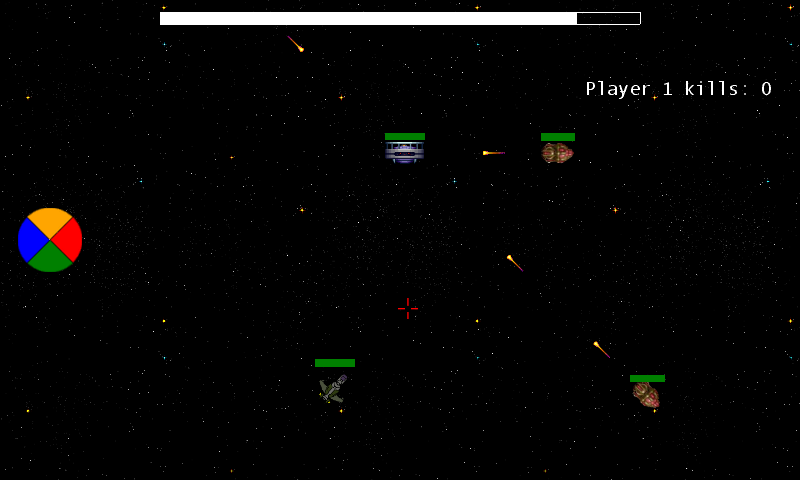
\includegraphics[width=\linewidth]{graphics/ingame}
    \caption{KJ-map of positive elements}
    \label{fig:poskjmap}
    \end{center}
\end{figure}

The first figure\ref{fig:poskjmap} is the KJ-map of the positive elements 
we identified during our PMA. We identified four major groups of elements.
They are as follows:

\begin{itemize}
    \item Final result
    \item Course related issues
    \item Group dynamics
    \item External tools and factors
\end{itemize}

As can be seen from the maps, we feel our choice of tool-chain and
process management was good. The team had experience with git, and using
github simplified many of the coordination-related issues we encountered.

The group worked very well together, and we were all enthusiastic about
the game we were making. Having only three members had its upsides, as it
simplified cooperation and management.

When it comes to the course-related issues, we have some complaints, but
there was still some positive notes.  We feel the structuring of the
documents we had to produce was good, and very much enjoyed the possibility
to get some practical experience.

We are of course also proud of the final result, although we wished to
have some more time for polish.

\subsection{Negatives}
\begin{figure}
    \begin{center}
    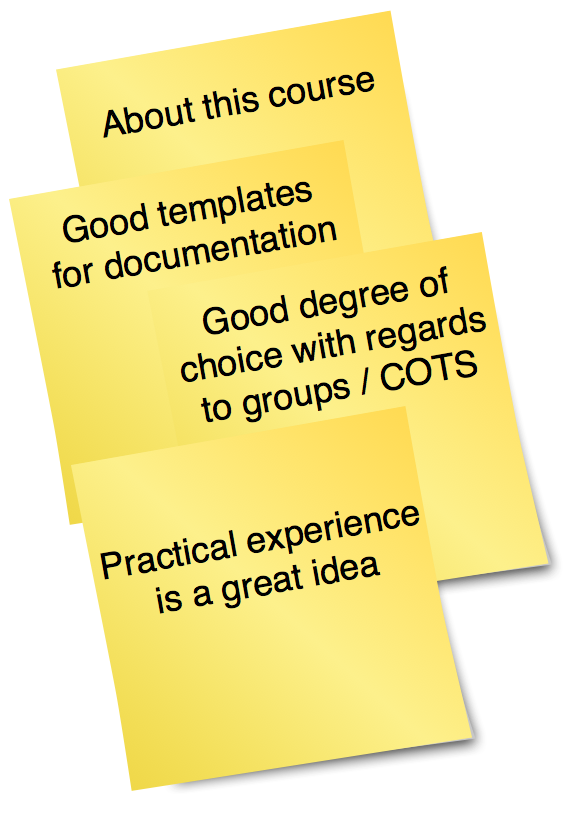
\includegraphics[scale=0.4]{graphics/postit/POS_about_course}
    \caption{KJ-map of negative elements}
    \label{fig:negkjmap}
    \end{center}
\end{figure}

\begin{figure}[ht]
    \begin{minipage}[b]{0.5\linewidth}
        \centering
        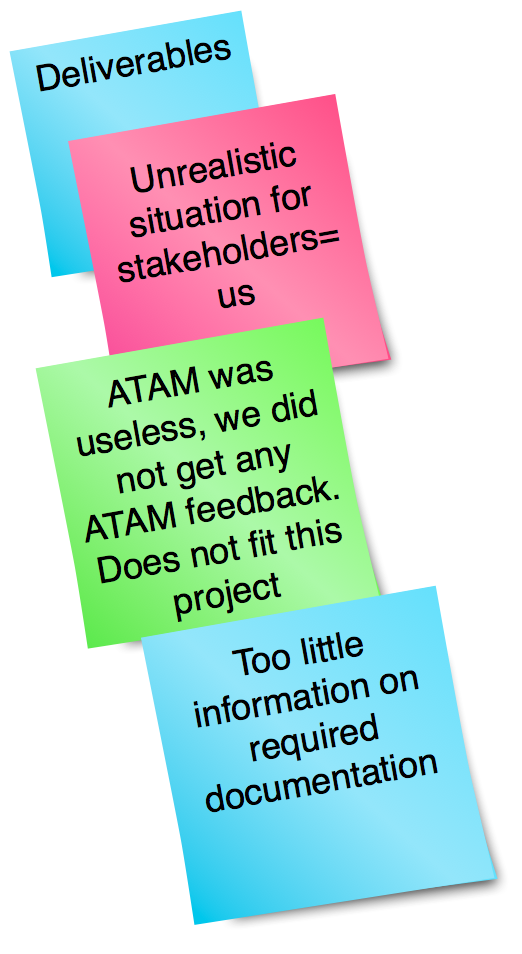
\includegraphics[scale=0.4]{graphics/postit/NEG_deliverables}
        \caption{Deliverables}
        \label{fig:neg1}
    \end{minipage}
    \hspace{0.5cm}
    \begin{minipage}[b]{0.5\linewidth}
        \centering
        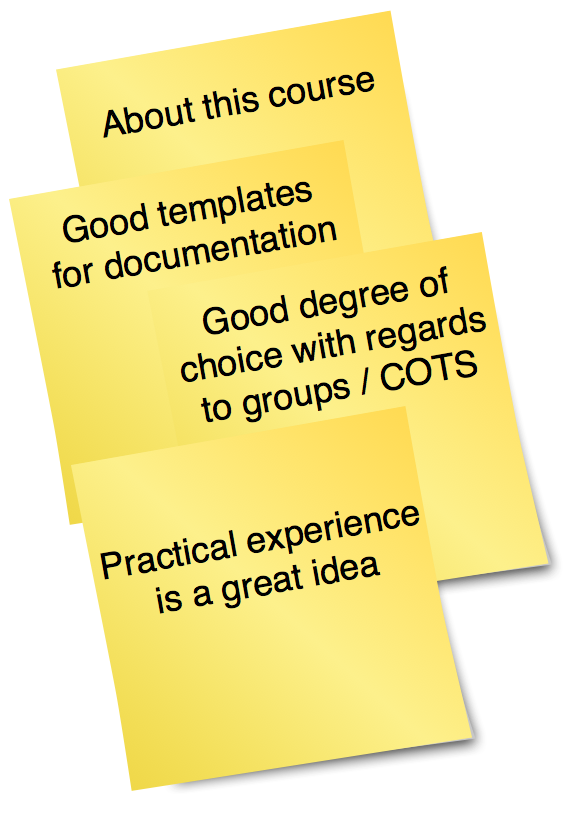
\includegraphics[scale=0.4]{graphics/postit/POS_about_course}
        \caption{Something}
        \label{fig:neg2}
    \end{minipage}
\end{figure}

For the negative elements we also identified four major groups:

\begin{itemize}
    \item Project management
    \item Deliveries
    \item Course-related
    \item Implementation issues
\end{itemize}

We started off slow in our group, as we had not agreed upon a game we all
wanted to make. I can only suspect the problems larger groups had with
this. As for us, we finally decided, and got started. By this time we had
already spent to much time for comfort, and had no plan for what was to
follow.  Throughout the project we were working with what our gut told us
was needed, and estimated deadlines on the fly. This was not optimal.

As for the deliveries, the documentation was in our view lacking. We felt
unsure of what we should include in each document, and felt there was no
natural order to things.

The ATAM process deserves special mention. We never received feedback from
either the opposing group, nor the course-responsible. The ATAM process in
itself was also not well suited to the way we, and the opposing group, had
documented our architectures.

We also feel the course could be reorganized somewhat. There was to little
time for actual implementation, and the design-process was drawn out.
The up-front exercises also did not teach us enough about XNA to get 
started. These could perhaps be run in parallel with the design phase.

Finally, our implementation was not perfect. The architecture we designed
was powerful, but also complex. We also had problems with getting artwork
for use in the game, and wound up relying on sources from the public
domain.

\section{Causal maps}

\subsection{Negative causal map}
We chose to focus on the time-crunch in our negative causal map. This was
the biggest issue in our view, and therefore deserving some extra focus.

\begin{figure}
    \begin{center}
    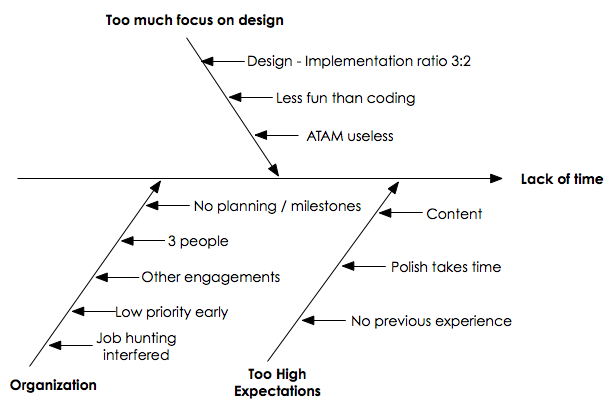
\includegraphics[width=\linewidth]{graphics/negMap}
    \caption{Negative causal map}
    \label{fig:negmap}
    \end{center}
\end{figure}

Identifying causes beyond the fact that we had only four weeks for 
implementation posed some problems, but we feel we have highlighted the
most important issues.

The most important issue was probably that we wanted too much. We had 
imagined the final game, and it was awesome. Then reality struck, and we
had to revise our expectations, but this happened on an intellectual level
rather than on an emotional level. We simply did not have the time or 
experience necessary to finish the project we had imagined.

We have already mentioned some organizational issues, and these probably
contributed to the lack of time. We all had other engagements which
received higher priorities. For instance we were all looking for jobs at
the time, and this took a lot of time.

Lastly, we spent to much time designing the architecture. The ratio of
design to implementation time is 3:2, which we feel is completely wrong.
If it were reversed we would be much happier.

\subsection{Positive causal map}

The thing we were most happy with in this project was the extensible
component-based system.  The causal map may not be a great fit for this,
but we want to highlight it in any case.

\begin{figure}
    \begin{center}
    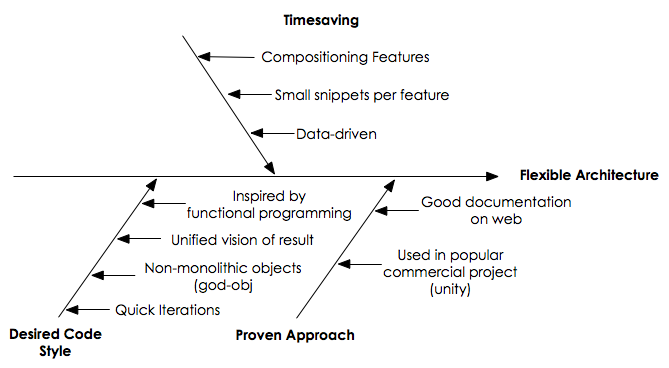
\includegraphics[width=\linewidth]{graphics/posMap}
    \caption{Positive causal map}
    \label{fig:posmap}
    \end{center}
\end{figure}

The system is our implementation of the well-known component-pattern from
the game industry. It has been implemented in AAA titles such as Prototype,
and is the basis for Unity3D, one of the most popular game engines today.

The architecture saved us incredible amounts of time when we had laid down
the basis. We could implement new features in a single function, and could
compose new features in data. This was a big boon to productivity.

We chose this approach because it is similar in style to functional 
programming, which the team have had good experiences with. It also saves
us from the dreaded \emph{God-object} which plagues many game 
architectures.

\section{Our experience of the PMA process}

The PMA got us thinking about our project from a non-code viewpoint, which
we needed. This was due to the fact that the diagrams were ill-suited to
implementation, and forced us to think along different lines.

The process was new and unexpected, but we feel that the graphical aids
(ie. KJ-diagrams and Causal maps) added complexity we could do without.
They are a lot of work, and a simple free-flowing discussion with a stated
purpose would work just as well.  The diagrams are also a poor method of
communicating ideas, and would be worthless without this document explain
the process which produced them.

\printbibliography


\section{Revision history}

\begin{table}[H]
  \begin{tabular}{| c | c | c |}
    \hline
    0.1 & 11.04.2011 & Initial revision of this document. \\
    \hline
  \end{tabular}
\end{table}

\end{document}
	\bibliographystyle{plainnat}